% Source: Code/ML_overlay/ir_rgb_registration/paper/ml_overlay_report_materials/ir_rgb_registration_report/figures/fig_spatial_transformer.tex
\documentclass[tikz,border=10pt]{standalone}
\usepackage{tikz}
\usetikzlibrary{arrows.meta,positioning,calc,shapes.geometric}

\definecolor{garnet}{RGB}{115,0,10}
\definecolor{rose}{RGB}{204,46,64}
\definecolor{atlantic}{RGB}{70,106,159}
\definecolor{congaree}{RGB}{31,65,77}
\definecolor{horseshoe}{RGB}{101,120,11}
\definecolor{black90}{RGB}{54,54,54}
\definecolor{black50}{RGB}{162,162,162}

\begin{document}
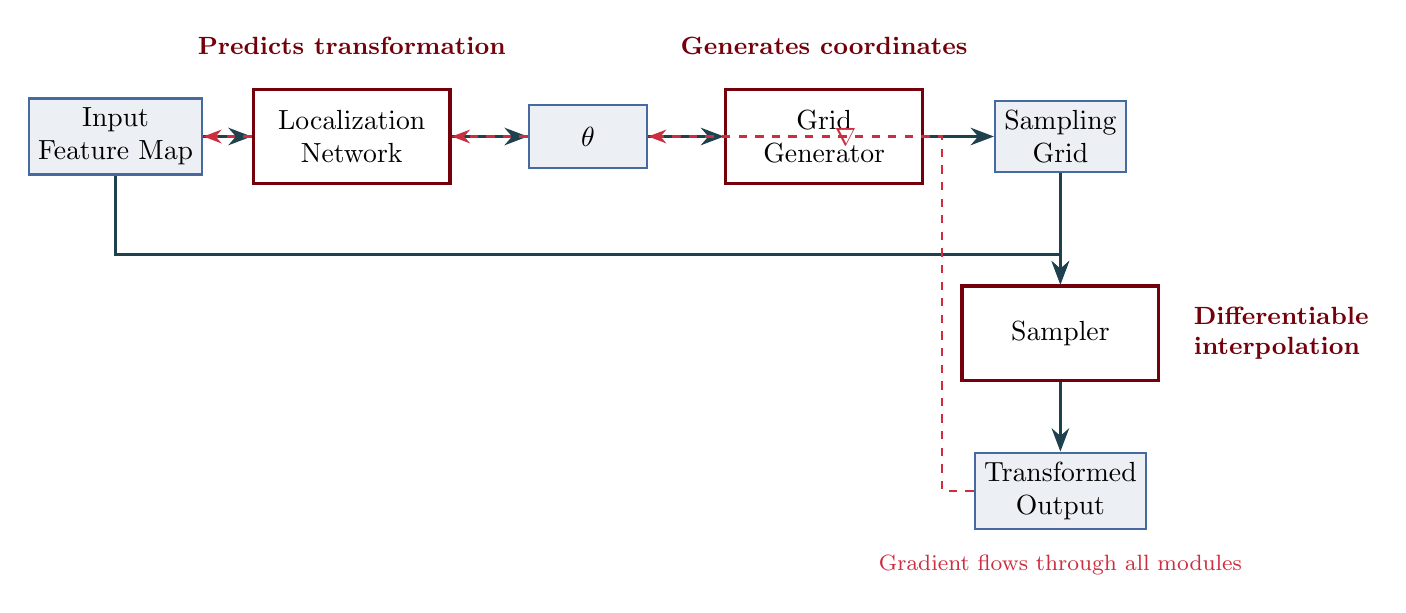
\begin{tikzpicture}[>=Stealth,
    box/.style={rectangle, draw=garnet, very thick, fill=white, minimum width=2.5cm, minimum height=1.2cm, align=center},
    data/.style={rectangle, draw=atlantic, thick, fill=atlantic!10, minimum width=2cm, minimum height=0.8cm, align=center},
    arrow/.style={->, very thick, congaree},
    gradient/.style={->, thick, dashed, rose}]

    % Input
    \node[data] (input) at (0,0) {Input\\Feature Map};

    % Localization Network
    \node[box] (loc) at (3,0) {Localization\\Network};

    % Transformation parameters
    \node[data, minimum width=1.5cm] (theta) at (6,0) {$\theta$};

    % Grid Generator
    \node[box] (grid) at (9,0) {Grid\\Generator};

    % Sampling Grid
    \node[data, minimum width=1.5cm] (sampgrid) at (12,0) {Sampling\\Grid};

    % Sampler
    \node[box] (sampler) at (12,-2.5) {Sampler};

    % Output
    \node[data] (output) at (12,-4.5) {Transformed\\Output};

    % Forward pass arrows
    \draw[arrow] (input) -- (loc);
    \draw[arrow] (loc) -- (theta);
    \draw[arrow] (theta) -- (grid);
    \draw[arrow] (grid) -- (sampgrid);
    \draw[arrow] (sampgrid) -- (sampler);
    \draw[arrow] (sampler) -- (output);
    \draw[arrow] (input) -- ++(0,-1.5) -| (sampler);

    % Gradient flow (backprop)
    \draw[gradient] (output) -- ++(-1.5,0) |- (theta) node[pos=0.7, right, font=\small, text=rose] {$\nabla$};
    \draw[gradient] (theta) -- (loc);
    \draw[gradient] (loc) -- (input);

    % Labels
    \node[above=0.3cm of loc, font=\small\bfseries, garnet] {Predicts transformation};
    \node[above=0.3cm of grid, font=\small\bfseries, garnet] {Generates coordinates};
    \node[right=0.3cm of sampler, font=\small\bfseries, garnet, align=left] {Differentiable\\interpolation};

    \node[below=0.2cm of output, font=\footnotesize, rose] {Gradient flows through all modules};

\end{tikzpicture}
\end{document}
